\documentclass{article}
\usepackage{polski}
\usepackage[utf8]{inputenc}
\usepackage{amsmath}
\usepackage{amsthm}
\usepackage{graphicx} 
\usepackage{hyperref}
\title{Algorytmy Genetyczne}
\author{Katarzyna Kosek}

\begin{document}
	\maketitle
	\newpage
	\pagenumbering{arabic}
	\section{Wykład 1}
		\subsection{Zasady zaliczenia.}
		2 kolokwia w semestrze, projekt 1 na 2 osoby, samemu trzeba wymyśleć temat do końca października. \textbf{Deadline na projekt:} dwa tygodnie przed końcem semestru.
		\\
						\textbf{KOLOKWIUM 1: 21 listopada} \\
						\textbf{KOLOKWIUM 2: 9 stycznia} 
		\subsection{Literatura}
		\begin{itemize}
			\item P. Goldberg - Algorytmy genetyczne i ich zastosowania - 50% materiału stąd
			\item	J. Arabas - Wykłady z algorytmów ewolucyjnych
			\item	Z. Michalewicz - Algorytmy genetyczne + struktury danych = programy ewolucyjne
			\item	J. Koza - Genetic Programming I - XII
		\end{itemize}
		\subsection{Historia}
		Algorytmy genetyczne powstały około roku 1960. Za pioniera badań uznaje się Johna Hollanda (u. w Michigan). Równolegle Igor Reichenberg( chyba) oraz Hans von coś tam (jakieś dziwne te nazwiska). Ci drudzy to bardziej strategie ewolucyjne.
		\paragraph{Algorytmy genetyczne}
		Algorytmy genetyczne są algorytmami procesu optymalizacji opartymi na zasadach doboru natrualnego oraz dziedziczenia. Wykorzystują mechanizmy adaptacyjne systemów biologicznych do tworzenia narzędzi informatycznych. 
		\paragraph{Elementarnym algorytmem genetycznym może być:}
		\begin{itemize}
			\item maksymalizacja funkcji - \\
		jest jakaś funkcja. Interesuje mnie jakieś maksimum funkcji w danej dziedzinie (powiedzmy $0<a<b$).
		
			\item Hifi (bez instrukcji obsługi) [Wypłata] - \\
		mam sobie skrzynkę, i ileś tam przełączników z dwoma możliwymi przełącznikami. 	Ze skrzynki wychodzi dźwięk XD Obserwujemy efekt ustawienia przełączników na 	output z systemu . Można zastosować kodowanie?
		
		\end{itemize}
		\subsection{Etapy algorytmu genetycznego:}
		\begin{itemize}
			\item \textbf{Kodowanie} - fenotyp $\leftrightarrow$ genotyp. Mamy znaleźć najlepszy fenotyp, najlepszą konfigurację dla Hifi. Rozwiązania poszukujemy nie w fenotypach, ale w genotypach. Musimy dokonać transkrypcji pomiędzy genotypem a fentypem. Trzeba znaleźć geny. \\
			Wybór genów:  skończna liczba symboli. W przypadku Hifi 0 i 1. W tym przypadku łatwo jest stworzyć chromosom. (kombinacja 0 i 1). \\
			Dla maksymalzacji można robić podobnie: 
			$0 < a < b$ - zapisać w postaci binarnej liczbę. I potem tym chromocomem jest liczba w postaci binarnej
			
			\item \textbf{Wybór populacji początkowej} - polega to na losowaniu zbioru ozdobników $ N > 50$
			\item \textbf{Tworzenie następnych populacji} - przebiega dzięki działaniu na populacjach naszych rozwiązań trzech operatorów. \\
			\begin{enumerate}
				\item \textbf{Operator reprodukcji (selekcja)} W sposób przypadkowy wybieram pewne elementy ze starej generacji. Najbardziej przekonywująca jest selekcja liniowa, wymaga ona tego aby $f(x) \Rightarrow 0$
				funkcja celu $\rightarrow f(x) \rightarrow$ ona ma być zmaksymalizowana
				Nie moze być ujemna - selekcja wykorzystuje "koło ruletki", operuje na prawdopodobieństwach.
				osobnik pierwszy zajmuje sektor  23\%, drugi 12\%. Tak robię z każdym z osobników. 
				Zakręcam ruletką, i patrzę na którego osobnika wskażę ruletka. Selekcja jest poprzez ruletkę. 
				W rezultacie lepsze osobniki mają szansę wprowadzenia do nowej populacji. Gorsze osobniki mogą być wogóle nie reprezentowane. \\
				Czasami trzeba coś dodać coś do funkcji, żeby prawdopodobieństwo nie było ujemne.
				\item \textbf{Cross-over} - kojarzenie w parach, to takie śmieszne cięcie
				\item \textbf{Mutacja} - randomowe zmienianie jakiś genów, jest jej kilka rodzajów, ogólnie polega na losowej zmianie poszczególnych genów. 
			
			
			\end{enumerate}
			\item  Iteracja etapu III aż do $ f_T(x_i)_i > C $
			\subparagraph{}
				\centering	max $f_T(x_i) > C $ \\
				$t>T$ (np. T=50) \\
				$\frac{f_{T-1}(x_i) - f_T(x_i)}{f_{T-1}(x_i)+f_T(x_i)_i} < \varepsilon$ \\
		\end{itemize}
		
	\section{Wykład 2}
	
	
		
		\subsection{Funkcja celu z jedną zmienną.}
		Funkcja celu:	$f(x_i) = x_i^2 $
		$$x_i \epsilon [0,1,2\ldots.1023] $$
		$$x_i \rightarrow genotyp = 010101 
		$$(w sumie 10 genów)
		allel =  0  lub  1
		$x_i = 7 \\
		x_i = 85 \\
		x_i = 524 \\
		x_i = 988 $ \\
		\\
		W funkcji przynależności:\\
		$
		f(85) = 7225 \\
		f(524) = 274516 \\
		f(988) = $ no bardzo dużo\\
		
		\paragraph{Ruletka.} Gdy narysuje się ruletkę, pierwsze dwie wartości są niewidoczne, 3 i 4 zdominują
		populacje. Dla tego specyficznego układu jest istotne, aby dla genotypu na
		pierwszym miejscu stała jedynka (kwestia postaci binarnej liczby, tam sobie można przeliczyć). 
		
		\subsection{Funkcja celu z dwiema zmiennymi.}
			\begin{equation*}
				f(x,y)=x^2+y^2 
			\end{equation*}
			\begin{equation*}
				x,y \epsilon [0,1023]
			\end{equation*}

		
		Na etapie krzyżowania na skutek interakcji genotypów mogą powstać
		słabsze geny.
		Aby tego uniknąć kopiujemy geny X i Y na zmianę. Z tego wniosek że dobrze by
		było tak zakodować gen aby geny które tworzą ważne cechy danego typu były położone blisko
		siebie - żeby były odporne na operator krzyżowania. 
		\\
		\\
		\paragraph {Istotne jest aby ważne cechy zapisywać za pomocą jak najmniejszej
		ilości genów.}
		\subsection{Jak kodować genotyp:}
		\begin{itemize}
			\item ważne cechy odpowiadają ważnym genom
			\item grupy powinny byc zwarte
			\item jeżeli ważne cechy mają być opisywane za pomocą genów, to tych genów
			powinno byc mało
		\end{itemize}
		\subsection{Podstawowe twierdzenie algorytmów genetycznych. Twierdzenie o schematach.}
		Schemat - wirtualny chromosom \\
		Zajmujemy sie genotypami z pojedynczych chromosomów. Na każdym miejscu
		może stać metasymbol bądz poligen, na przykład ${0xxxxx}$ lub
		${0xx01}$ (odpowiednio schemat $H_1$ i $H_2$). Można powiedzieć że chromosom
		reprezentuje dany schemat.\\ \\
		\textbf{l} - długość chromosomu \\
		\textbf{N} - populacja fenotypów  \\
		Każdemu chromosomowi odpowiada $2^l$ schematow. \\
		$N_H=N2^l-N+1$ (to odejmowanie wynika z permutacji z gwiazdkami) \\
		$2^l  < N_H < N(2^l-1)+1$ \\
		
		\subsection{Metoda enumeracyjna.}
		\subparagraph{}
		Sprawdzam wszystkie rozwiązania,
		szczególnie trudne dla wielu wymiarów, potem mogą podzielić na pół i sprawdzić
		gdzie jest lepiej, i tak dalej - dziwne. Dla 2 wymiarów dzielę na płaszczyzny,
		a dla 3 na sześciany? XD Efektywne dla niskich wymiarów, ale nie zawsze prowadzi
		do dobrych rozwiązań. 
		\subparagraph{} Jeśli $l>N$, ilość schematów jest większa niż ilość fenotypów tej
		populacji. Ilość przetwarzanych schematów jest przeważnie znacznie większa niż
		ilość fenotpów. Siłą algorytmów jest to, ze przetwarzają schematy a nie fenotypy
		i genotypy. Schematem zwycięzkim jest schemat majacy reprezentantów w populacji,
		i jest schematem którego ważne geny są blisko, ma mało ważnych genów. 
		\subparagraph{Jak zaprogramować algorytm genetyczny, nie znając genotypów?} Najlepszy
		jest najszybszy algorytm, który propaguje najlepszych osobników.
	\section{Wykład 3}
		$H = xx1x00x\\
		chromosom = 0010001$
		Jak zmienia się liczba schematów populacji o indeksie t\\
		$m(H,t+1)=?$\\
		\subsection{Etapy, operatory}
			\paragraph{ Etap Selekcji } $f(H)$ jest wybierany z prawdopodobieństwem $\frac{f(H)} {\Sigma f_i} = P_j(H)$ - prawdopodobieństwo wylosowania do następnej populacji osobnika z indeksem j\\
			$m_j=P_j(H)N=\frac{f_i(H)}{\frac{1}{N}\Sigma f_i}=\frac{f_i(H)}{F_j(t)}$ \\
			$m = \Sigma m_j = \frac{\Sigma f_j(H)}{f_j(t)}$ średnia po i, nie wiem jaki jest znaczek XD\\
			
		
			Średnie przystosowanie osobników reprezentujące schemat H jest >= od średniego przystosowania przeciętnego osobnika populacji.
			\subsubsection{Etap (operator) krzyżowania} 
			\textbf{Rozpiętosć schematu} - odległość skrajnych ustalonych genów - $\delta(H)$\\
			$\delta (xx00xxxx)=1$\\
			$\delta (1xxxxxx0)=7$\\
			$p_c = 0,7 - 0,8 $- operator krzyżowania\\
			$l=8$ - długość chromosomu\\
			Oszacowujemy prawdopodobieństwo zniszczenia - $1 - \delta(H) over l-1 p_c$ \\
			\subsubsection{Etap mutacji}
			xxxxxx - działanie jakiegokolwiek operatora na ten schemat nic nie zmieni\\
			xx00011 - tu będziemy mieć problem, schemat może nie przejść do następnej populacji, aby przeszedł do następnej populacji $(1-p_m)^{O(H)} w przybliżeniu 1-O(H)p_m$ - prawdopodobieństo tego, że dany schemat prezjdzie dalej \\
			\textbf{Rząd schematu} - O(H)- liczba ustalonych genów \\
			Występuje preferencja dla schematów których ustalone geny są blisko \\
			Do następnej generacji są preferowane cegiełki które są schematami o małym O(H), małym l(H) i przedstawiające \textbf{ważną cechę} \\
			\textbf{Metaalgorytm genetyczny} - próbujemy różnych cech na oślep i patrzymy co się dzieje - wtedy kiedy nie wiemy które cechy są ważne, stosujemy to kiedy nie wiemy kiedy $p_c$ i $p_m$ maja optymalne wartości \\
			Mamy problem, kiedy osobnikiem jest algorytm, krzyżujemy algorytmy i próbujemy znaleźć optymalne wartości parametrów.
			
		
		
		\subsection{Semantyka}
	$	\begin{array}{cc}
			\textbf{Genetyka} & \textbf{Informatyka} \\ 
			chromosom & ciąg kodowy \\ 
			gen, cecha & znak, detektor \\ 
			allel & wariant cechy \\ 
			genotyp & struktura \\ 
			fenotyp & rozwiązanie, zbiór parametrów
		\end{array} $
		\subsection{Uwagi ogólne:} 
		\paragraph{Algorytmy genetyczne:}
		\begin{itemize}
			\item nie przetwarzają bezpośrednio parametrów zadania ale jego zakodowaną postać (genotyp/fenotyp)
			\item działają na populacji rozwiązań
			\item korzystają z funkcji celu $f(x)$ i nie wymagają znajomości pochodnych funkcji celu
			\item stosują kombinacje metod deterministycznych i \textbf{probabilistycznych}
			\item nie dostarczają rozwiązań idealnych ale lepsze niż średnie
			
		\end{itemize}
		Jeśli dla danego problemu mam metodę szczególną (wyspecjalizowaną) dla tego problemu to będzie ona miała przewagę nad nad algorytmem genetycznym\\
		$f(x) = W_5(x)$ - wzory Viete'a\\
		Gdy nie jesteśmy pewni którego stopnia jest wielomian, lepsze są algorytmy genetyczne.
		\subsection{Metody optymalizacji}
			\paragraph{Metody analityczne}
			\begin{itemize}
				\item Metody pośrednie : pochodna po funkcji równa zeru (szukanie maksimum bądź minimum danej wielkości) - nie zawsze funkcja jest analityczna, nie zawsze można liczyć pochodne
				\item Metody bezpośrednie : metody maksymalnego gradientu, wadą jest znajdowanie ekstremów lokalnych, rozwiązanie: zastosowanie kilku różnych warunków początkowych
			\end{itemize}
			\paragraph{Metody enumeratywne (przeglądowe)} Jak znaleźć maksimum funkcji w dziedzinie $(x_1 , x_2)$, ogólnie dzielenie na podprzedziały, metoda może być łatwo "zwiedziona", przy dużej ilości parametrów obliczenia robią się strasznie złożone numerycznie, można zwiększyć prawdopodobieństwo udziału zwiększając liczbę przedziałów, lecz to zwiększa znacznie złożoność obliczeń
			\subsection{Algorytmy genetyczne a teoria dwurękiego bandyty}
			Dwa miejsca na pieniążki, mogę ciągnąć za prawe bądź lewe ramię, na dole wychodzi wypłata. W jednym z kasyn jest automat, który rzekomo daje więcej wygranych dla jednego ramienia, ale nie wiemy które. Adaś ma N żetonów po 1 złoty. \\
			$2n<N$ - faza nauczania (eksploracji, poznawania - n żetonów na lewe, n żetonów na prawe)\\
			$N>(N-2n)\rightarrow0$\\
			Należy zdecydować ile wynosi n małe - zoptymalizować to.\\
			$\mu _1, \mu _2$ - średnie wygrane na ramieniu 1 i 2\\
			$q(n)$ - prawdopodobieństwo tego że po fazie eksploracji n+n gorsze ramię dało lepszy wynik\\
			$L(N,n)$ - strata wynikająca z przyjętej strategii w porównaniu do strategii opartej na pełnej informacji \\
			$\mu _1 > \mu _2 \rightarrow L(n,N)=(\mu _1 - \mu _1)[n+(N - 2n)q(n)]$ \\
			Należy obliczyć prawdopodobieństwo podjęcia złej decyzji \\
			$P(x_1)=\frac{1}{\sqrt{2\pi}\sigma _1}exp[-\frac{1}{2\sigma^2_1}(x_1 - \mu _1)^2]$ \\
			$P(x_2)=1\rightarrow2\\
			P(nx_1) \mu_1 \rightarrow n\mu_1\\ \sigma_1 \rightarrow \sqrt{n}\sigma_1$
		\section{Wykład 4}
			Sens porównywana bandyty jest w tym, że to jest podobne do algorytmu genetycznego \\
			Faza eksperymentu $\rightarrow$ Faza eksploracji \\
			Najpierw mamy 2n prób, potem sprawdzamy. Jest tam także równanie na stratę: 
			$$L(N,n)=(\mu_1-\mu_2)[(N-n)q(n)+n(1-q(n))]$$
			Prawdopodobieństwo można oszacować za pomocą rozkładu Gaussa
			$$N(\mu_2, \sigma^2_1)$$
			$$N(\mu_2, \sigma^2_1)$$
			Bądź za pomocą rozkładu Goldberga:
			$$q(n)=\frac{1}{\sqrt{2\pi}}\frac{e^{\frac{x^2}{2}}}{x}$$
			$$x=\frac{\mu_1-\mu_2}{\sqrt{\sigma_1^2 + \sigma_2^2}}\sqrt{n}$$
			$$\int_{x}^{\infty}\frac{1}{\sqrt{2\pi}}e^{t^2/2}dt < \int_{x}^{\infty}\frac{t}{x}\frac{1}{\sqrt{2\pi}}e^{t^2/2}dt$$
			$u=e^{\frac{t^2}{2}}$ \\
			$du = -te^{\frac{t^2}{2}}$ \\
			$$\frac{1}{\sqrt{2\pi}}\int_{x}^{\infty}\frac{t}{x}e^{-\frac{t^2}{2}}dt=
			\frac{1}{\sqrt{2\pi}x}\int_{x}^{\infty}te^{-\frac{t^2}{2}}dt=
			\frac{1}{\sqrt{2\pi}x}\int_{-x^2/2}^{0}du=
			\frac{1}{\sqrt{2}\pi x}e^{-\frac{x^2}{2}}$$
			Prawdopodobieństwo oszacowania wyniku da się opisać ogonem rozkładu Gaussa
			Dla nas najważniejsze jest to, jaka jest optymalna liczba prób.
			Trzeba obliczyć optymalną liczbę prób za pomocą... 
			\\ obrazek \\
			$$c=\frac{\mu_2-\mu_1}{\sqrt{\sigma_1^2+\sigma_2^2}}$$
			Optymalny podział prób polega na tym że liczba prób z lepszym ramieniem rosła szybciej niż wykładniczo.
			Powinniśmy rozpatrywać problem k-ramiennego bandyty.
			Naszym k-ramiennym bandytą jest pewna liczba konkurujących schematów - są to takie schematy gdzie na każdej pozycji dla i $\epsilon 1,2,...l$ że
			$$a_i = b_i = * \oplus
			a_i \neq *, b_i \neq *, a \neq b_i$$
			\paragraph{Przykłady} dla l=7 \\
			**00*0**\\
			**00*1**\\
			**01*0**\\
			Przykład schematów konkurujących na pozycjach 2, 3, 5. Konkurują one o przydział ważnych cech w populacji. Prawidłowa strategia wymaga żeby przydział miejsc dla najlepszych schematów rósł szybciej niż wykładniczo. Tu jest ta analogia do k-ramiennego bandyty. Schematy genetyczne będą konkurowały żeby przetrwać do następnej generacji. 
			\paragraph{Ograniczenia algorytmu genetycznego}
			\begin{itemize}
				\item Chcemy zrozumieć źródła trudności, na jakie może napotykać się algorytm genetyczny elementarny
				\item Można stworzyć jakieś proste zagadnienie gdzie dojdzie do takiej sytuacji gdzie nasz algorytm genetyczny będzie rozmijał się z globalnym optimum - gdzie np. znajdzie optimum lokalne.
				\item Chcemy naruszyć "hipotezę cegiełek".
			\end{itemize}
			
			\subparagraph{Hipoteza cegiełek}dobrze przystosowane schematy niskiego rzędu małej rozpiętości grają kluczowa rolę w tworzeniu i działaniu AG.
			\subparagraph{Problem rzędu 2 (problem dwubitowy)} Mamy cztery schematy, każdy z nich ma pewną funkcję przystosowania f: \\
			
			$$***0***0* - f_{00}$$\\
			$$***0***1* - f_{01}$$\\
			$$***1***0* - f_{10}$$\\
			$$***1***1* - f_{11}$$\\
			$F_{11}$ jest globalnym optimum. $f_{11} > f_{10}, f_{11} > f_{01}, f_{11} > f_{00}$
			
			\subparagraph{}Problem zaczyna się wtedy, gdy wprowadzimy element \textbf{zwodniczości}: jeden lub oba schematy rzędu 1 mające suboptymalnych reprezentantów są lepsze niż odpowiedni schemat rzędu 1 mające optymalnych reprezentantów.
			
			$$f(0*)>f(1*) \\ / f(*0)>f(*1)$$
			To jest kwestia schematów, a nie konkretnych przypadków!
			\subparagraph{} Goldberg w swojej książce dowiódł że tam nie ma lub, tylko jest albo. 
			$$\frac{f(01)+f(00)}{2} > \frac{f(10)+f(11)}{2}$$
			Powyższa równość jest prawdziwa, jeśli liczba populacji danych schematów jest równa. 
			$$\frac{f(00)+f(10)}{2} > \frac{f(01)+f(11)}{2}$$
			Jeśli dodamy dwie nierówności stronami:
			$${2f(00)+f(01)+f(11)}>2f(11)+f(01)+f(10)$$
			z czego wychodzi:
			$$f(00) > f(11)$$
			Unormujmy wszystko:
			$$r = \frac{f_{11}}{f_{00}}, c=\frac{f_{01}}{f_{00}}, c'=\frac{f_{10}}{f_{00}}$$
			Globalność/Zwodniczość
			$$r>1,c,c'$$
			
			$$r < 1+c-c' \equiv f_{11} < f_{00} + f_{01} + -f_{10}$$	
			$$f_{11}+f_{10}<f_{00}+f_{01} \implies$$
			$$c-c' >0 \implies c>c' \implies f_{01} > f_{10}$$	
			$$r<1-c' + c \implies 1-c'>0 \implies c'<1  \implies f_{10} < f_{00}$$
			$$\implies$$
			$$f_{10}<f_{01}, f_{00}$$			
			\subparagraph{Przypadek 1} $c>1 \equiv f_{01} > f_{00}$ - łatwiejsze do rozwiązania
			\subparagraph{Przypadek 2} $c<1 \equiv f_{01} < f_{00}$ - trudniejsze do rozwiązania
			\subparagraph{Rysunek - problem zwodniczy}
			$$f_{0*}>f_{1*}$$ Funkcja f nie jest liniowa. Geny oddziaływują ze sobą.
			$$f(x_1, x_2)=ax_1 + bx_2 + c + dx_1x_2 $$
		\section{Wykład 5}
			Misleading problems for genetical algorythms. We have the scheme:
			$$f_{11}>f_{00}, f_{01}, f_{10}$$
			$$f_{x1} < f_{x0}$$
			Now it could be altough the solution (blue eyes, blonde hair) is not hte perfect solution.
			Analytic description of this issue: Lets consider following table: destruction and creation of ...
			If I combine two such skills:
			\paragraph{}
			
			\begin{center}
				$\begin{array}{ccccc}
				\centering
				& 00 & 01 & 10 & 11 \\ 
				00 & S & S & S & 01,10 \\ 
				01 & S & S & 11,00 & S \\ 
				10 & S & 00,11 & S & S \\ 
				11 & 01,10 & S & S & S
				\end{array} $
			\end{center}
			
			
			
			
			 $$[\frac{12}{16}]_s, [\frac{3}{4}]_s$$
			 
			$$$$
			$$p_{00}^{t+1}=p^t_{00}\frac{f_{00}}{f}
			[1-p'\frac{f_{11}}{f}p^t_{11}]
			+p_c'\frac{f_{01}f_{10}}{f_2}
			+ p_{01}^tp_{10}^t$$
					(neglecting mutation)
					
			rozpiętość chromosomu:
			$$p_c'=p_c\frac{\rho(H)}{l-1}$$
			
			$$p^{t+1}_{01}=p^t_{01}\frac{f_{01}}{f}
			[1-p'_c\frac{f_{10}}{f}p^t_{10}]
			+p_c'\frac{f_{00}f_{11}}{f_2}
			+ p_{00}^tp_{11}^t$$
			
			$$p^{t+1}_{10}=p^t_{10}\frac{f_{10}}{f}
			[1-p'_c\frac{f_{01}}{f}p^t_{01}]
			+p_c'\frac{f_{00}f_{11}}{f_2}
			+ p_{00}^tp_{11}^t$$
			
			$$p^{t+1}_{11}=p^t_{11}\frac{f_{11}}{f}
			[1-p'_c\frac{f_{00}}{f}p^t_{00}]
			+p_c'\frac{f_{01}f_{10}}{f_2}
			+ p_{10}^tp_{01}^t$$
			
			$$[(00)(11)], [(01)(10)]$$
			Numerical simulations of misleading scenario:
			if $p_{ab}^{t=0}>0$ then $p_{11}^{t=\infty}=1$ \\
			\paragraph{}
			Schemat komplementarny 00 może zdominować populację jeśli jest wystarczająco dużo jego reprezentantów w populacji początkowej $t=0$.
			\begin{figure}[ht]
				\label{fig:fig1}
				\centering
				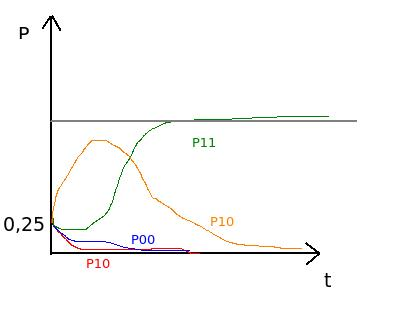
\includegraphics[scale=0.4]{wyk5.jpeg}
				\caption{Schemat komplementarny}
			\end{figure}
			\\ rysunek 3d: dla schematu (0,*,0) - 2D - linia \\	
			
						\begin{figure}[ht]
							\label{fig:fig1}
							\centering
							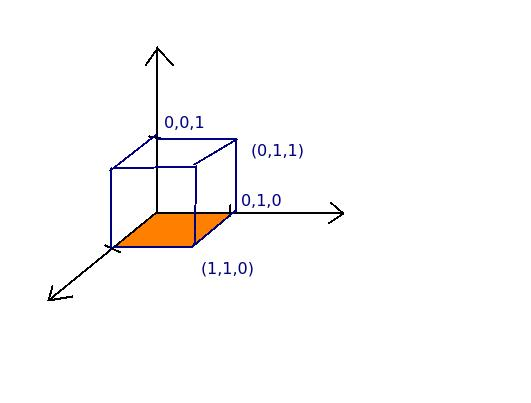
\includegraphics[scale=0.4]{3dwyk5.jpeg}
							\caption{Schemat}
						\end{figure}
						
			Każdy schemat rzędu 3 jest punktem.\\
			Każdy schemat rzędu 2 jet prostą. \\
			Każdy schemat rzędu 1 jest płaszczyzną (**0) (pomarańczowa na rysunku).
			\\ Każdy schemat rzędu 0 - cała przestrzeń. Gdy mamy coś dowodzić z AlGenów możemy częściowo korzystać z algebry która operuje na przestrzeniach hiperwymiarowych.
			\paragraph{Przekształcanie funkcji celu}
			
				\begin{figure}[ht]
					\label{fig:fig2}
					\centering
					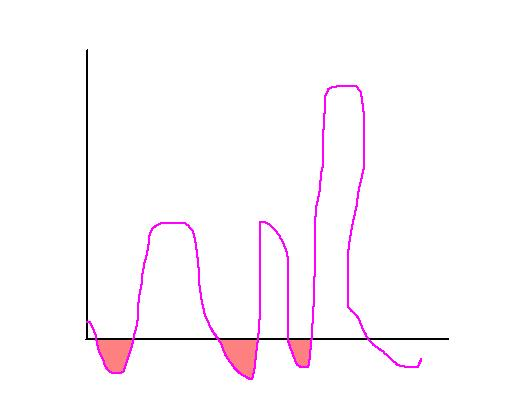
\includegraphics[scale=0.5]{ujemna_funkcja_celu.jpeg}
					\caption{Ujemna funkcja celu}
				\end{figure}
				
				$$x_i^{t=0}, i=1,..N$$
				$$[f(x_i^{t=0})]_{min}=<=$$
				$$f\rightarrow\hat{f} + |c|$$
				Czyli po prostu dodaję stałą, tylko nie za dużą. Dotyczy to tylko i wyłącznie problemu ruletki. 
				$$f_i > \bar{f}$$
				Selekcja liniowa wybiera poprzez prawdopodobieństwo $\frac{f_i}{\bar{f}}$
			\subparagraph{Inne metody selekcji}
				\begin{itemize}
					\item Selekcja turniejowa - wybieram 1 lub 2 najlepszych, robię kolejny turniej, i znowu wybieram najlepszych za pomoca funkcji przynależności	
				\end{itemize}
			Problem optymalizacji $f(x)=min$, $\hat{f}(x)=-f(x)$, max$\hat{f}(x)$
			\subparagraph{Skalowanie czasowe}
			Na początku selekcja powinna być łagodna: dodawanie dodatniej stałej do funkcji celu aby nie pozwolić na tzw. \textbf{przedwczesną zbieżność}. W innym przypadku znajdujemy się w maksimum lokalnym a nie globalnym.
				
				\begin{figure}[ht]
					\label{fig:fig2}
					\centering
					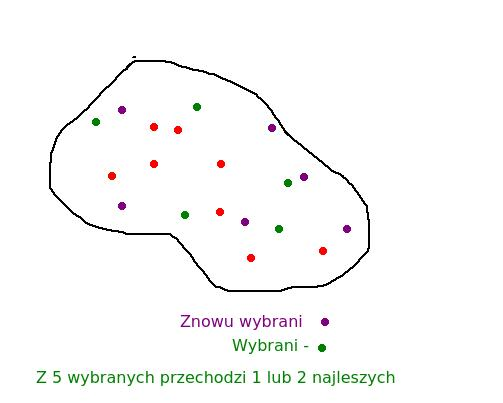
\includegraphics[scale=0.5]{selekcja_turniejowa.jpeg}
					\caption{Selekcja turniejowa}
				\end{figure}
				
			Na końcu powinna być selekcja wzmocniona: potem mamy bardzo małe różnice pomiędzy osobnikami, zależy odjąć jakąś stałą dodatnią: $\hat{f}=f-const$
			Renormalizacja polega na zmianie funkcji: $\hat{f} = af+b$
			
						\begin{figure}[ht]
							\label{fig:fig1}
							\centering
							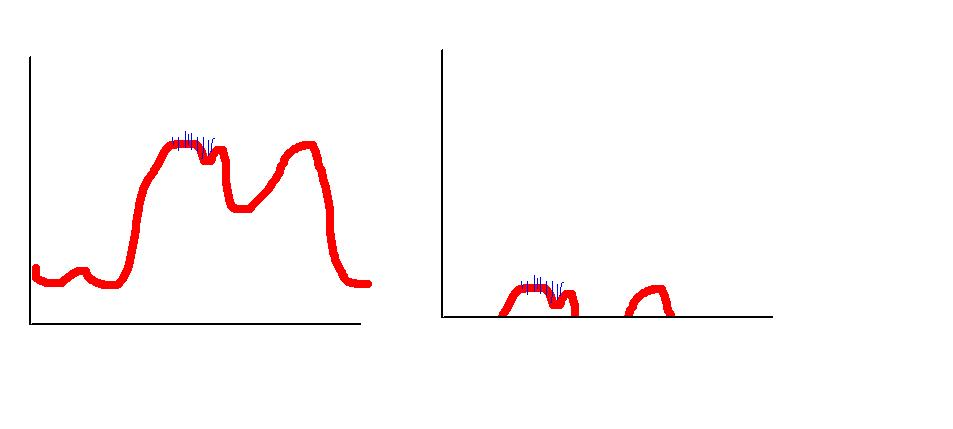
\includegraphics[scale=0.4]{selekcja_wzmocniona.jpeg}
							\caption{Selekcja wzmocniona}
						\end{figure}
	\section{Wykład 6}
		\paragraph{Kodowanie diploidalne}
		Fenotyp zależy od genotypu w którym są dwa komplety genów potrzebnych do stworzenia genotypu. Reguła ekspresji - który z genów jest brany pod uwagę aby w organizmie pojawiła się jakaś cecha. Załóżmy, że jeżeli są dwa różne geny, to ujawnia się gen pisany dużą literą, np. A, czy tam D. A jak są dwie małe, ujawnia się mała litera (gen recesywny).
		
		\begin{figure}[ht]
			\label{fig:fig2}
			\centering
			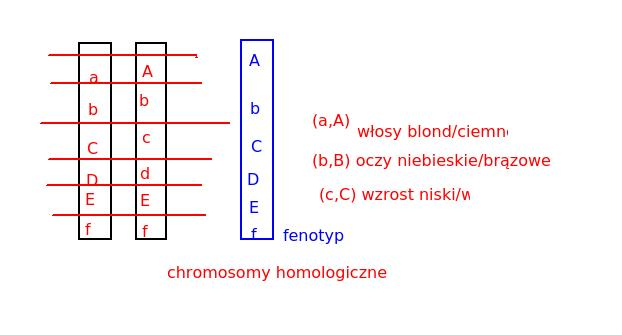
\includegraphics[scale=0.5]{homologiczne.jpeg}
			\caption{Chromosomy homologiczne}
		\end{figure}
		
		\subparagraph{} Większość tego co omawialiśmy odpowiada haploidom - pojedyncze chromosomy (nie ma chromosomów homologicznych). Haploidy to np. glony. Wszystkie wyższe organizmy są diploidami. Po co natura wymyśliła kodowanie diploidalne? Bo pozwala ona na lepszą adaptację do \textbf{zmieniającego} się środowiska. Znany jest przyadek wszy której gen recesywny zmienił się na dominujący, zmieniła ona barwę skrzydeł, jest to związane ze zwiększonym zanieczyszczeniem atmosfery. 
		\subparagraph{} Dlaczego one maja większą zdolność do przystosowania się? W materiale genetycznym mogą być przechowywane recesywne geny które się nie ujawniają, ale są przechowywane w każdym osobniku. Jeżeli w środowisku zajdzie zmiana, i a będzie bardziej korzystne niż A, wystarczy zmienić mechanizm ekspresji, albo poczekać aż będą się spotykały a małe dwa razy w trakcie crossing-over. Wtedy taki osobnik ma dużą siłę fenotypu i poprzez operator selekcji może silnie zdominować populację. Częściej - zmiana charakteru genu. 
		\paragraph{Kodowanie przykładowe}Geny funkcyjne ${0,1}$, geny modyfikatory ${m,M}$ - decydują o dominacji. Jak to będzie wyglądać? W fenotypie dominuje gen 0 gdy przynajmniej w jednym z chromosomów homologicznych jest jeden  gen M.
		\subparagraph{} $\begin{array}{|c|c|c|c|c|}
			& 0M & 0m & 1M & 1m \\ 
			0M & 0 & 0 & 0 & 0 \\ 
			0m & 0 & 0 & 0 & 1 \\ 
			1M & 0 & 0 & 1 & 1 \\ 
			1m & 0 & 1 & 1 & 1
		\end{array}$ 
		\subparagraph{Kodowanie trialleliczne} Geny : ${0,1,2}$. Jedynka jest recesywna, 2 jest dominująca nad 0. Ekspresji unika cecha w fenotypie {0,1} \subparagraph{}
		$\begin{array}{|c|c|c|c|}
			& 0 & 1 & 2 \\ 
			0 & 0 & 0 & 1 \\ 
			1 & 0 & 1 & 1 \\ 
			2 & 1 & 1 & 1
		\end{array} $
		\paragraph{Praktyka - porównanie działania hoploidy i diploidy}
		Zagadnienie plecakowe - celem znalezienie jest takiego zbioru i żeby suma po tym zbiorze była największa.
		\begin{figure}[ht]
			\label{fig:fig2}
			\centering
			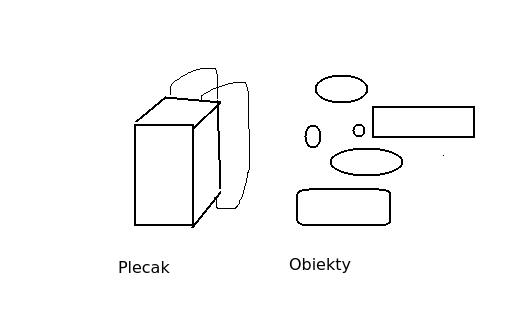
\includegraphics[scale=0.5]{plecak.jpeg}
			\caption{Zagadnienie plecakowe}
		\end{figure}
		'$$I={i}=?$$
		$$\Sigma_{I} w_i = max$$
		a - masa, b - objętosć
		$$\Sigma_{I} a_i < A$$
		Suma atrybutów typu a musi być mniejsza od jakiejś krytycznej wiekości.
		$$\Sigma_{I} b_i < B$$
		No i wybieramy te elementy za pomocą algorytmów genetycznych.
		Szukamy zbioru indeksów II które spełniają tę cechę. Wyobraźmy sobie ze to zagadnienie jest \textbf{zmienne w czasie}. Pewne cechy będą się zmieniały w czasie. Inne rzeczy w zimie, inne w lecie XD. 
		$$w_i(t)$$
		Rozwiązujemy ten problem za pomocą algorytmu genetycznego. zmiana środowiska ma dramatyczne efekty dla doskonałości funkcjonowania populacji. 
		
				\begin{figure}[ht]
					\label{fig:fig2}
					\centering
					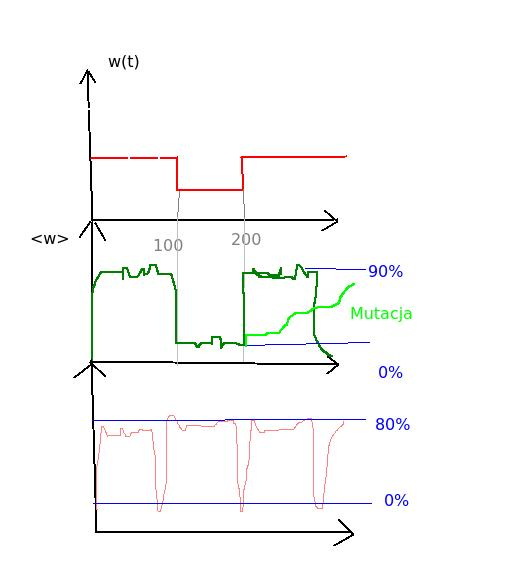
\includegraphics[scale=0.5]{diplohaplo.jpeg}
					\caption{Średnie przystosowanie populacji dla haploid i diploid}
				\end{figure}
				
		\paragraph{Podstawowe twierdzenie AG dla diploid} Załóżmy żę: $$H_0=**0*$$
		$$H_1 **1* \\ f(H_0) = f_d \\ f(H_1)=f_r$$
		$$f_r < f_d \\ 1 - recesywna$$
		Diploidalność pozwala na pozostawienie pewnej puli recesywów.
		pt - prawdopodobieństwo recesywu\\
		$$p^{t+1}=\frac{(p^t)^2f_r+p^t(1-p^t)f_d}{(p^t)^2f_r+[1-(p^t)^2]f_d} K$$
		$\uparrow$ mutacja pominięta \\
		Mianownik - średnie przystosowanie populacji\\
		Licznik - $[1-(p^t)^2]f_d$ - efekt maskowania \\
		K - wpływ krzyżowania na mutację  $$K = 1 - p_c\frac{\delta(t)}{l-1}- o(H)\frac{p}{m}$$
		$$p_t << 1$$ więc
		$$p^{t+1}=\frac{p^tf_dK}{1* f_d} \approx p_tK$$
		$$\frac{p^{t+1}}{p^t}\lim\limits_{t\rightarrow \infty} \rightarrow K\approx 1$$
		\subparagraph{Haploidy:}
		$$p^{t+1} = \frac{p^tf_r}{p^tf_r + (1-p^t)f_d}K$$
		$$p^t<<1$$
		$$\frac{p^tf_r}{f_d}K$$
		$$\frac{p^{t+1}}{t} przy t << 1 = \frac{f_r}{f_d} << 1$$
		Geny są gubione dużo szybciej niż dla diploid.
		$$r=\frac{f_d}{f_r}$$
		$$\frac{p^{t+1}}{pt}= \frac{1}{p^t + (1-p^t)r}$$
		\subparagraph{Diploidy:}
		$$\frac{p^{t+1}}{p^t}=\frac{p^t + (1 -p^t)r }{(p^t)^2 + (1-p^t)^2r}$$
		
		\subparagraph{}
		\begin{figure}[ht]
			\label{fig:fig2}
			\centering
			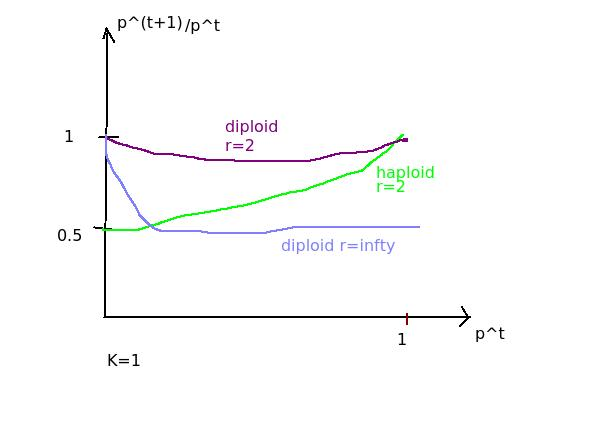
\includegraphics[scale=0.5]{wyk6_pt1pt.jpeg}
			\caption{Iloraz dla haploid i diploid}
		\end{figure}
		Im większe jest R, tym większe jest to zagłębienie. Dla $r \rightarrow \infty$ 
		$$\frac{p^{t+1}}{p^t}=\frac{1-p^t}{1-(p^t)^2}=\frac{1}{1+p^t}$$
		Długookresowa pamięć - polega na tym, że $$\frac{p^{t+1}}{p^t}$$ dla diploidów jest znacznie większe niż dla haploidów.
		\subparagraph{}
		$$p^{t\rightarrow \infty}, p_m>0$$
		Haploid: $$p^{t+1} = (1-\epsilon)p^t + p_m(1-p^t)-p_mp^t$$
		$$p^{t+1}=p^t=p^\infty = ?$$
		$$\epsilon p^t = p_m(1-2p^t)$$
		$$p^t(\epsilon+2p_m)p_m$$
		$$p^t = \frac{p_m}{\epsilon+2p_m} \approx \frac{p_m}{\epsilon}$$
		Prawdopodobieństwo recesywu proporcjonalne do prawdopodobieństwa mutacji. 
		\subparagraph{Rewolucja recesywów dla diploidów}
		\begin{itemize}
			\item $p^{t+1} = (1 -\epsilon)p^t + p_m(1-p^t)-p_mp^t$ , $p^{t=\infty}\sim p_m$
			\item dla diploidów: $p^{t+1}=(1-2\epsilon p^t)p^t + 2p_m(1-p^t) - 2p_mp^t$
		\end{itemize}
		
		Prawdopodobieństwo utworzenia genu recesywnego dla genu jest określone przez człon $(1-2\epsilon p^t)p^t$
		
		$$p^{t+1} \approx p^t$$
		$$2\epsilon (p^t)^2 = 2p_m(1-2p^t) \approx 2p_m$$
		$$p_{\infty} prpoporcjonalne \sqrt{p_m} $$
		
		\section{Wykład 7}
		\paragraph{Niestandardowe operatory genetyczne}
		\subparagraph{Operator duplikacji} $$D_b[AbcDE] = AbbcDE$$
		\subparagraph{Operator delecji} $$\bar{D_b}[AbbcDE] = AbcDE$$
		\subparagraph{Operator inwersji}: zmiana kolejności genów $$$$
		\begin{itemize}
			\item Inwersja liniowa: w chromosomie rysujemy dwa punkty  (be) i ten segment jest odwrócony$$AbcDeF \rightarrow AeDcbF$$
			\item Inwersja boczna: polega na tym że losuję jeden punkt (pomiędzy D i e) $$AbcDeF \rightarrow DcbAFe$$
			\item Inwersja liniowo-boczna: z prawdopodobieństwem 0,75 inwersja liniowa, z prawdopodobieństwem 0,25 inwersja w stosunku do każdego z boków 
		\end{itemize}
		
		Po co takie operatory w przyrodzie? Ważne funkcjonalnie cechy powinny być kodowane w cegiełkach, w zestawach krótkich. Jeżeli jakaś cecha ma być zakodowana w genach A i D to musi być jakiś operator pozwalający na ruch genów, w ten sposób operator krzyżowania ma małą szanse rozbijania cegiełki. \\
		Powstaje problem: gdy zaczynamy krzyżować dwa osobniki z których jeden został poddany inwersji a drugi nie: 
		$$ABc|De$$
		$$AbE|dc$$
		z tego powstają:
		$$ABcde$$
		$$AbEDe$$
		No i osobniki są nieżywotne. :(
		Żeby sobie z tym poradzić, trzeba zdefiniować przykładowo metodę \textbf{kojarzenie według wzorca}. Najpierw tworzymy jakiś wzorzec kolejności genów, i geny w obu chromosomach ustawiamy wg tego wzorca. Tym wzorcem bardzo często jest osobnik o większej funkcji celu. 
		\paragraph{Problem różnicujący (?) płeć}Mamy dwie czynności istotne dla tworzenia potomstwa: h - hunting, n - nursing. Prawdopodobieństwo przeżycia potomstwa - S(n,h).
		Jaka jest funkcja opisująca S?
		\paragraph{Haploidy}
		$$h + n + ahn = 1$$
		$$h = \frac{1-n}{1+an}$$
		$$S = \frac{n(1-n)}{1+an}=^{max}$$
		$$a=0 \implies n=\frac{1}{2}$$
		$$n \pm = \frac{-1 \pm \sqrt{1+a}}{a}$$
		w granicy
		$$\frac{-1 +1 +\frac{1}{2}}{a} = \frac{1}{2}$$
		\section{Wykład 8}
		
		$n$ - wychowanie\\
		$h$ - polowanie\\
		
		$$n + h + anh = 1$$
			
		$$ S(n,h) = nh= n h(n) = \frac{n(1-n)}{1+an} $$
		
		$$ \frac{\partial S}{\partial n} = \frac{(1+an)(1-2n) - n(1-n)a}{(1+an)^2} $$
		
		$$ 0 = 1-2n+an-2n^2a-an+an^2 $$

		$$1-2n-n^2a=0 $$

		$$n^2a+2n-1=0$$

		r.kwadratowe

		$$n = \frac{-1 \pm \sqrt{1+a}}{a} =_{a \rightarrow 0} = \frac{1}{2}$$

		$$(n_1 , h_1) (n_2 , h_2)$$

		$$n_i + h_i + an_ih_i=1$$

		$$h_i=\frac{1-n_i}{1+an_i}$$

		$$S(n_1,n_2)=\frac{1}{2} (n_1+n_2)(2-n_1-n_2)$$

		dla $a = 0$
		$$
		\frac{\partial S}{\partial n_1} = \frac{1}{2} (2-n_1-n_2) - (n_1 + n_2) = 1-n_1-n_2
		$$
		
		$$1-n_1-n_2=0$$

		$$n_1+n_2=1$$
		
		dla $a \neq 0$
		$$
		\frac{\partial S}{\partial n_1} =0 \frac{\partial S}{\partial n_2} =0
		$$
		Nie ma rozwiązania dla $n_1 \in [0,1]$
		Wniosek: 
		max $S(n_1,n_2)$ jest dla brzegów przedziałów.\\
		$n_1 = 0 $\\
		$n_2 = 0$
		
		genotyp $\rightarrow$ fenotyp\\
		Problem komiwojażera\\

		$$T \sim e^{aN}$$
		
		Fenotyp = trasa\\
		1,2,4,5,3 <- miasta\\
		4 3 2 1 <- kolejność odwiedzania miast\\
		W tym przypadku odwiedzamy najpierw miasto 4 w kolei (czyli 5), wykreślamy je, odwiedzamy 3 w kolei z pozostałych 1,2,4,3 czyli 4, potem miasto drugie z 1,2,3 czyli 2 potem pierwsze z 1,3 czyli 1, a zostaje jedno(3). Ostatecznie chromosom 4 3 2 1 reprezentuje trasę 5$\rightarrow$4$\rightarrow$2$\rightarrow$1$\rightarrow$3\\
		Reprezentacja porządkowa WZORZEC 1 2 3 4 5 6 7\\
		Chromosom: ciąg liczb naturalnych 2 5 1 1 3 2\\
		Otrzymujemy trasę 2 6 1 3 7 5 4\\
		Problem $\rightarrow$ brak cegiełek
		\paragraph{PMX, partialy matched crossover}
		\url{https://www.youtube.com/watch?v=c2ft8AG8JKE} $\rightarrow$ znacznie prostszy sposób, trywialny do zrozumienia, polecam ^^
		2 osobników\\
		984 567 1320\\
		\textbf{871 230 9546}\\
		2 miejsca krzyżowania\\
		984 \textbf{230 1320}\\
		Tylko nie mogą się powtarzać niektóre liczby więc \textit{podążamy w tył} i 3$\rightarrow$6, 2$\rightarrow$5 0$\rightarrow$7\\ 
		Otrzymujemy:\\
		984 230 1657\\
		Dla drugiego chromosomu:\\
		801 567 9243 $\leftarrow$ analogiczne rozumowanie\\
		
		\paragraph{Metoda CX cycling crossover}
		\url{https://www.youtube.com/watch?v=85pIA2TYsUs} $\rightarrow$ świetne tłumaczenie\\
		Przykład z zajęć:
		\begin{table}
			\begin{tabular}{c|c|c|c|c|c|c|c|c|c|c}
				C=	&9	&8	&2	&1	&7	&4	&5	&0	&6	&3\\
				D=	&1	&2	&3	&4	&5	&6	&7	&8	&9	&0\\
				C'=	&9	&2	&3	&1	&5	&4	&7	&8	&6	&0\\
				D'=	&1	&8	&2	&4	&7	&6	&5	&0	&9	&3\\
			\end{tabular}
		\end{table}
		
		Systemy klasyfikacyjne, układ poszukujący reguł, klasyfikatorów
		\begin{enumerate}
			\item Układ przetwarzania komunikatów
			\item Układ oceniający
			\item AG
		\end{enumerate}
		\textbf{\textit{1}} Jest szczególną wersją systemu produkcji\\
		produkcja $\rightarrow$ jeśli $<$warunek$>$ to $<$akcja$>$ \\
		produkcja - zestaw reguł\\
		jeśli $<$warunek$>$ to $<$akcja$>$ - klasyfikator $\rightarrow$ jedna reguła \\
		Klasyfikator:\\
		$<$warunek$>$ : $<$komunikat$>$\\
		jeśli warunek \{0,1,\#\}$^l$ to komunikat \{0,1\}$^l$
			
		\section{Wykład 9}
		
		Systemy liczenia maszynowego. Klasyfikatory. $\leftarrow$ w poprzednim tygodniu
		Jeżeli wszystkie klasyfikatory mogą zawierać głos i przetwarzać informacje to nie jest to dobre dla systemu. Tak jak np wszyscy mówią i jest przypał, nikt sę niczego nie dowie. To od razu sugeruje że są równi i równiejsi. Są klasyfikatory gorsze i lepsze. Należy wprowadzić:
		$$S_i(t)$$
		To jest siła klasyfikatora. Należy wprowadzić system rozliczeń pomiędzy klasyfikatorami - brygada kubełkowa. Opiera się na następujących regułach:
		\begin{itemize}
			\item za zabranie głosu trzeba płacić, siła się zmniejsza jeżeli klasyfikator jest biedny, i wcześniej zabierał głos
			\item za prawidłowe zabranie głosu jest nagroda - tzn. jeżeli ktoś zabierze głos z sensem i wszyscy z tego skorzystają to ta osoba będzie nagrodzona.
			\item za milczenie też trzeba płacić (obecność w systemie)
			\item klasyfikatory bardziej specyficzne powinny mieć pierwszeństwo
		\end{itemize}
		To się sprowadza do:
		$$S_i(t+1)=S_i(t)+R_i(t)-C_{bid}\delta*S(t)-C_{tax}S_i(t)$$
		$C_{bid}$ - podatek obrotowy \\
		$\delta _t$ - w przedziale {0,1} \\
		$C_{tax}$ - podatek który się zawsze płaci \\
		\paragraph{}
		
		\begin{center}
		
	$	\begin{array}{cccccccccc}
			\# klasyfikatora  & \textbf{Siła} & \textbf{klasyfikator} & \textbf{Komunikat} &  \textbf{Oferta} \\
			1 & 200 & 01\#\#,0000  & - & 20 \\ 
			2 & 200 &  00\#0,1100 & - &  & \\
			3 & 200 &  11\#\#,1000 & - &  & \\  
			4 & 200 &  11\#\#,1000 & - &  & \\
		\end{array} $
		
		$\begin{array}{cccc}
		\text{Siła} & \text{Komunikat} & \text{Dopasowanie} & \text{Oferta }\\ 
		 178 & 0000 & -   \\ 
		 198 &  1000 & 19.8 \\ 
		 198 &  & -   \\ 
		 198 &  & -   \\ 
		\end{array} $
		
		
	$	\begin{array}{cccc}
		\text{Siła} & \text{Komunikat} & \text{Dopasowanie} & \text{Oferta }\\ 
			215.8 & - &  &  \\ 
			178.2 & 1100 &  &  \\ 
			196 & - & 2 & 19.6 \\ 
			178.2 & 0001 & 2 & 17.8
		\end{array} $
		
	$	\begin{array}{cccc}
		\text{Siła} & \text{Komunikat} & \text{Dopasowanie} & \text{Oferta }\\ 
			213,6 & - & - & - \\ 
			213.8 & - & - & - \\ 
			174.4 & 1000 & 2 & 17.4 \\ 
			158.4 & 0001 & 2 & 15.8
		\end{array} $
		
		$\begin{array}{cccc}
		\text{Siła} & \text{Komunikat} & \text{Dopasowanie} & \text{Oferta }\\ 
					211.5 & - & - & - \\ 
					244.9 & - & - & - \\ 
					155.3 & - & - & - \\ 
					140.6 & 0001 & 3 & 14.0
				\end{array} $
				
		\end{center}
		
		\paragraph{} Środowisko chciało nagrodzić ekspertów, i te +50 trafia do ostatniego klasyfikatora.
		
		\begin{center}
	$	\begin{array}{c}
			\text{Siła} \\ 
			209.3 \\ 
			242.5 \\ 
			153.7 \\ 
			175.4
			\end{array} $
		\end{center}
			
		$$S(t+1)=S(t)[1 - C_{bid}\delta(t)-C_{tax}]+R(t)=
		S(t)[1-K(t)] + R(t)$$
		$$<\delta (t)>C_{bid}=\hat{C}_{bid}$$
		$$S(n) = (1-\hat{K})^nS(0)+\Sigma^{n-1}_{j=0}R(j)\hat{(1-K)}^{n-j-1}$$
		
		$$S(n)=S(n+1)=S_{ss}$$
		$$S(t)\hat{K} = R(t) \rightarrow R_{ss}$$
		$$S_{ss}\hat{K}= R_{ss}$$
		$$S_{ss}=\frac{R_{ss}}{\hat{K}} \rightarrow 
		B_{ss}=C_{bid}, C_{tax}* S_{ss}\delta(t)=C_{bid}<\delta(t)S_{ss}=C_{bid}<\delta(t)>\frac{R_{ss}}{\hat{K}}$$
		
		\paragraph{}Trenując klasyfikatory na danych populacjach po jakimś czasie, i po takim czasie gdy osiąga stan stacjonarny, działamy algorytmem genetycznym.
		
		%$$Z_0^1^T \rightarrow Z_0^T$$
		Algowytm genetyczny włączamy co ileś iteracji z otoczeniem.
		Krzyżowanie: 01\#\#0|001, \#\#001|001
		\subparagraph{}Selekcja nie powinna być silnie destruktywna. Wybiera się przeważnie jakiś procent reguł, np. $G = 0.1$ i wybiera się N*G reguł które poddaje się działaniu tych trzech operatorów: ruletka, krzyżowanie, mutacja. Szukamy reguł podobnych wśród N. Dziecko wyprodukowane w ten sposób powinno zająć miejsce kogoś kto jest zbliżone do niego. Zamiana AG z klasyfikatorami najbardziej podobnych. Jeżeli jest bliski rodzicowi, to zamieniamy.
		\subparagraph{Hierarchia domniemań}
		\#\#\#\#:0000\\
		1101:0011	\\
		Enviroment: $\langle 1101 \rangle$
		Ten pierwszy będzie zawsze się odzywał, drugi jest zgodny na 100 \% z pierwszym. Najpierw przyznaje się prawo bardziej szczegółowym klasyfikatorom, gdy jest kolizja opinii, przyznaje się miejsce tym dokładniejszym. Oferta klasyfikatora powinna być mnożona przez specyficzność klasyfikatora - A + liczba miejsc ustalonych.
		
		\section{Wykład 10}
		\paragraph{Hierarchie domniemań} Im reguła jest \textbf{bardziej} szczegółowa, tym powinna być \textbf{ważniejsza}.
		\paragraph{Mulitiplekser}Dwie szyny adresowe, 4 szyny przesyłu danych\\
			\begin{figure}[ht]
				\label{fig:fig2}
				\centering
				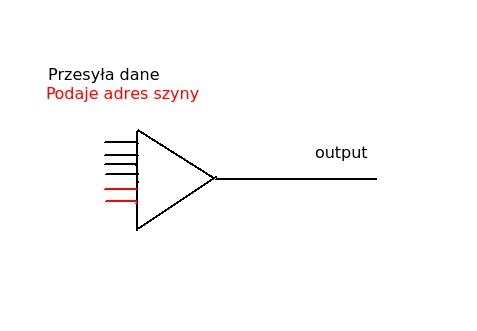
\includegraphics[scale=0.5]{multiplekser.jpeg}
				\caption{Multiplekser}
			\end{figure} 
		$$D_3, D_2, D_1, D_0, A_1, A_0 : output $$
		$$***000:0$$
		$$***100:1$$
		$$**0*01:0$$
		$$**1*01:1$$
		$$*0**10:0$$
		$$*1**10:1$$
		$$0***11:0$$
		$$1***11:1$$
		Działanie elementu można zapisać za pomocą ośmiu klasyfikatorów. Mogę wprowadzić pewien wynalazek w którym liczba reguł jest mniejsza. Ten wynalazek to hierarchia domniemań. 
		$$B_i=C_{bid} f(S_p)S_i$$
		$S_P$ - szczegółowość wzorca, liczba 0 i 1 we wzorcu (regule)
		$$f(S_p)=C + S_p$$
		Stałą wprowadza się bo jeżeli klasyfikator nie zawierałby żadnych reguł żeby miał też jakąś szansę.\\
		4 reguły  $$......  : 0$$
		Reguła nr 9	$$******:1$$
		Układ składający się z 5 reguł ma działać reprezentując multiplekser. Jeżeli uwzględnimy że siła 9 reguły to C, $f_1=f_2=f_3...c+3$
		\subparagraph{}Wewnętrzna pamięć systemu może pomieścić tylko jeden komunikat. Jeśli jest sygnał który pasuje do każdej z reguł 1-4, to z uwagi na ich siłę jedno z nich prowadzi sygnał do outputu. Jeśli jest sygnał pasujący do 2,4,6,8 to zadziała reguła 9, i nie ma ona żadnej konkurencji. Wstawiamy reguły 1,3,5,7 + 9 bez hierarchii domniemań.
		
		\begin{figure}[ht]
			\label{fig:fig2}
			\centering
			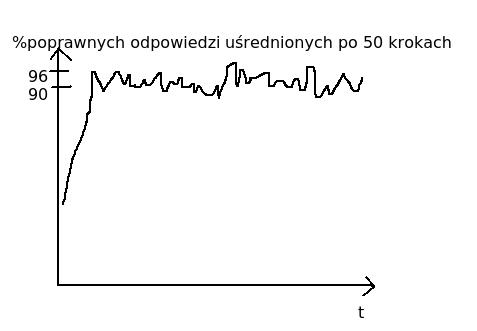
\includegraphics[scale=0.5]{bezhierarchii.jpeg}
			\caption{Procent poprawnych outputów bez hierarchii domniemań}
		\end{figure}
		
		\begin{figure}[ht]
			\label{fig:fig2}
			\centering
			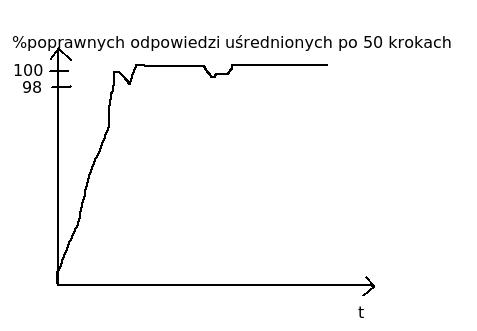
\includegraphics[scale=0.5]{zhierarchia.jpeg}
			\caption{Procent poprawnych outputów z hierarchią domniemań}
		\end{figure}
		
		\paragraph{} Jest możliwe 1458 reguł.
		Siła reguł do uczenia maszynowego jest to, że ich nie znamy, i musimy je odkryć. Co trzeba zrobić, to ze zbioru wszystkich reguł wylosować np. 100 reguł. Większość z nich prawdopodobnie jest zła, nawet nie oddziaływują ze sobą, ale mogą ze sobą konkurować, i to robią aby określić działanie multipleksera.
		
		\begin{figure}[ht]
			\label{fig:fig2}
			\centering
			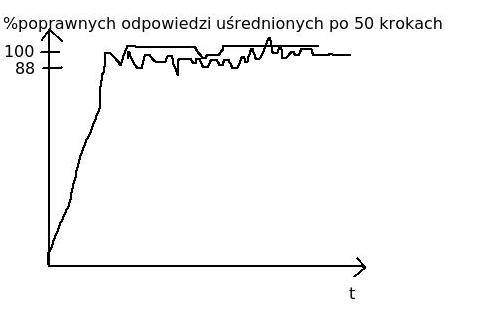
\includegraphics[scale=0.5]{bezalgen.jpeg}
			\caption{Hierarchia domniemań bez algorytmów genetycznych}
		\end{figure}
		
		\begin{figure}[ht]
			\label{fig:fig2}
			\centering
			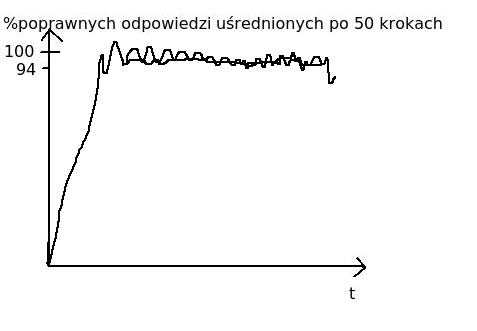
\includegraphics[scale=0.5]{algenhier.jpeg}
			\caption{Hierarchia domniemań z algorytmami genetycznymi}
		\end{figure}
	 
		\paragraph{Strategie ewolucyjne} Rozwiązywanie problemu optymalizacji części samolotu 
		\begin{itemize}
			\item brak genotypu, ewolucja bezpośrednia fenotypu
			\item kluczowa rola mutacji
		\end{itemize}
		 Szukam pewnego rozwiązania które zapisuję jako wektor $\vec{x}\epsilon R^k$
		 $$\vec{x}_{t+1} = \vec{x}_t + \vec{\eta}_t, \{\vec{x}_t, \vec{x}_{t+1}\}$$
		Wybieram lepszego osobnika. Musimy manipulować poziomem szumu, który zależy od t. Bierze się on z 
		%$$P(\eta_t^{(1)})=\frac{1}{\sqrt{2\pi}\sigma_t^{(1)}
		%	exp\{\frac{[\eta_t^{(1)}]^2}{2[\sigma_t^{(1)}]^2}\}$$
		\paragraph{Reguła 1/5 sukcesu} Jeśli w l kolejnych generacjach t liczba mutacji zakończonych sukcesem (dziecko jest lepsze od rodzica) jest większa niż 1/5 l to należy zwiększyć siłę mutacji. W przypadku jednowymiarowym oznacza to że 
		$$\sigma_t \rightarrow c_i\sigma_t$$
		$$c_i = \frac{1}{0,82}\approx1,22$$
		$$\sigma_t \rightarrow \sigma_t = c_d$$
		$$c_d = 0,82$$
		
		\paragraph{}SE ($\mu + \lambda$) - ta jest bardziej zachowawcza niż następna 
		\paragraph{}SE ($\mu, \lambda$) - Możemy wybierać rozwiązania z większej grupy populacji. Mamy $\mu$ osobników początkowych oraz $\lambda$ dzieci i wybieramy $\mu$ spośród $\mu + \lambda$ osobników. Lepsza jest turniejowość, z tej grupy wybieram podgrupę kilka razy. Selekcja jednokrokowa, bądź selekcja turniejowa.
		$$\lambda > \mu$$
		Selekcja tylko spośród dzieci.
		$$P(\eta_t^{(1)}, \eta_t^{(2)}) = 
		\frac{1}{2\pi \sigma_t^{(1)}\sigma_t^{(2)}}
		exp[ - \frac{\eta_t^{(1)}}{2}]$$
		No ogólnie wzór na dwuwymiarowego gaussa, taki potworek.
		No tutaj to ewidentnie dobrze to od kogoś przepisać.
		\paragraph{Krzyżowanie}
		
		\subparagraph{A}
		$$\vec{x}_1, \vec{x}_2$$
		$$\vec{x}_t^{(1)} = a\vec{x}_t^{(1)} + (1-a)\vec{x}_t^{(2)}$$
		$$\vec{x}_t^{(2)} = a\vec{x}_t^{(2)} + (1-a)\vec{x}_t^{(1)}$$
		$$\vec{\sigma}_t^{(2)} = a\vec{\sigma}_t^{(2)} + (1-a)\vec{\sigma}_t^{(1)}$$
		
		\subparagraph{B} 
		$$[x_t^{(1)}, n]' = x^{(1)}_t$$	dla n=2,5,12,34...
		Dla n $\notin \Omega$
		$$[x_t^{(1)}, n]' = x^{(2)}_t$$
		
		\section{Wykład 11}
		Mutacja mutacji $$\sigma(t \rightarrow \sigma(t+1)=\sigma(t)e^{\eta(t)}$$
		$$P(\eta(t))=\frac{1}{2\pi}e^{-\frac{\eta^2}{2}}$$ 
		Szczególnie się nadają do sytuacji gdy mam rozwiązanie problem wektorów jakiś tam. 
		\paragraph{Programowanie genetyczne} Idea rozwijana przez jakiegoś Johna Kozę, w skrócie chodzi o wykorzystanie algorytmu genetycznego do pisania programu. Osobnikiem nie jest liczba bądź wektor, ale jest nim program. No w zasadzie to optymalizuje. Do tego celu wykorzystuje się język LISP. Formalna składnia tego języka opiera się na nawiasach. Tworzymy pewien zbiór symboli "atomy", np. liczba 37, operator +, albo jakiś string. Pewne z atomów odgrywają rolę terminali - takich inputów ewentualnie outputów. Atomy mogą tworzyć listy które mogą zawierać atomy i inne listy. Przykładowo listą będzie:
		\begin{itemize}
			\item $L_1 =$(+3,7) - działanie 3 + 7
			\item $l_2 = y -x$
			\item *$L_1, L_2$ - mnożenie L czyli $*(+37)(-xy)$
			\item $L_4$ = NOT A
		\end{itemize}
		
		To wszystko można przedstawić jako drzewa: \\
				\begin{figure}[ht]
					\label{fig:fig2}
					\centering
					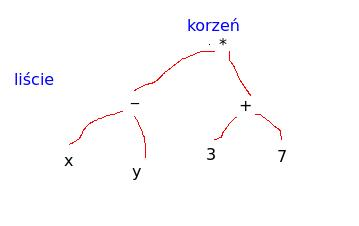
\includegraphics[scale=0.5]{drzewowosc.jpg}
					\caption{Hierarchia domniemań bez algorytmów genetycznych}
				\end{figure}
		Chcemy żeby liście zawierały jak najwięcej inputu. Operator może być również operatorem przesunięcia w czasie : $x(t) \rightarrow x(t - \tau)$
		Załóżmy że naszym programem jest funkcja: 
		$$\sqrt{x^2+y^2}$$
		Atomy to $$\{ x,y,\sqrt{},+ ,* \, =\}$$
		Losuję populację osobników początkowych:
		\begin{itemize}
			\item losowanie populacji początkowej 
			\item krzyżowanie - polega na tym że bierzemy wszystko co jest pod jakimś węzłem i wymieniamy na inny węzeł.
			\item mutowanie
		\end{itemize}
						\begin{figure}[ht]
							\label{fig:fig2}
							\centering
							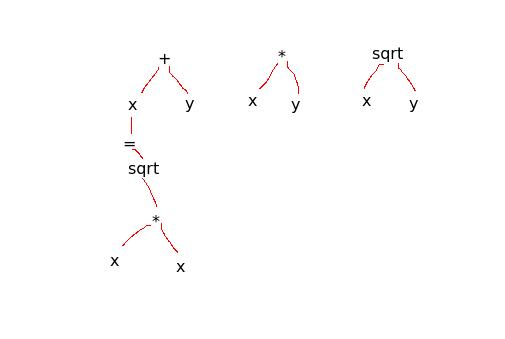
\includegraphics[scale=0.5]{prog_gen_losowanie.jpeg}
							\caption{Losowanie poszczególnych elementów}
						\end{figure}
		\subparagraph{}POdczas trzech operacji powstają osobniki nieżywotne, które trzeba usuwać. 
		Program napisany w LISPie może procesować program napisany w LISPie. 
		\paragraph{Choroby genetyczne} Model Penny chorób dziedziczonych genetycznie starzenie się organizmu.
		\paragraph{Hipotezy śmierci na skutek wieku}
		\begin{itemize}
			\item Ubytki telomerów
			\item Niszczenie DNA
			\item Ciągłe mutacje niszczą genetyczne niszczą nasz organizm, przenoszą się z pokolenia na pokolenie i ujawniają się gdy organizm przekracza pewien wiek.
		\end{itemize}
		Prawo Gampesa - Mortality rate - liczba $q(a)$ - prawdopodobieństwo zgonu dla osobnika który dożył a+1. \
		$q(a) prop exp(ba)$ 
		$N(a) -$liczba osobników w wieku a
		$$q(a)=\frac{N(a+1)-N(a)}{N(b)} \approx \frac{d[ln(N(a))]}{da}
		\approx \frac{lnN(a)-lnN(a+1)}{1}$$
		
		\paragraph{}
			\begin{figure}[ht]
				\label{fig:fig2}
				\centering
				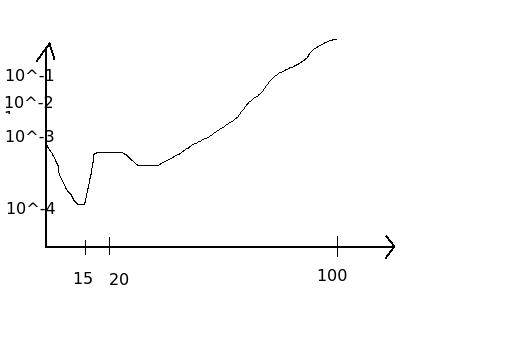
\includegraphics[scale=0.5]{umieralnosc.jpeg}
				\caption{Umieralność}
			\end{figure}
		 
		 $$q(a)=Aexp[b(a-x)]\approx11+-2$$
		 $$b>0\approx\frac{0,1}{rok}$$
		$$x =102,103$$
		
					\begin{figure}[ht]
						\label{fig:fig2}
						\centering
						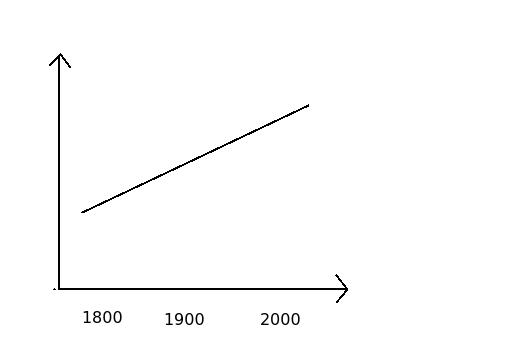
\includegraphics[scale=0.5]{stalab.jpeg}
						\caption{Stała b na przestrzeni wieków}
					\end{figure}
		Model Penny'ego zakłada ze każdy z nas ma genom w postaci 32 bitów. Jeden bit - jeden rok życia. Jeśli bit jest równy 1, to w danym roku ujawnia się choroba która będzie męczyła osobnika do końca jego życia. Osobnik umiera, jeśli liczba ujawnionych jedynek osiąga pewną krytyczną wartość. Aby osobnik żył, w chwili t to $$\Sigma_{\tau=1}^{t}b_\tau <  T$$ 
		Trzeba założyć że osobnik który dożywa wieku B w najprostszym przypadku płodzi przez kopiowanie swojego chromosomu o tym samym składzie genetycznym. Najsłabsze osobniki z dużą ilością jedynek nie przeżyją do momentu rozmnażania, więc się nie replikują.
		 Przy przekazywaniu materiału genetycznego zachodzą mutacje $\{0 1 \}$ (wyczerpywanie isę zasobów naturalnych). 
		$$V = 1 - \frac{N(t)}{N){max}}$$ - prawdopodobieństwo przeżycia.
		
		\section{Wykład 12}
		\paragraph{Zastosowanie algorytmów genetycznych w sztucznych sieciach neuronowych}
		
		Neurony: warstwowe i nie. Wszystkie wagi otrzymuje się metodą wstecznej propagacji błędu. W ostatnich latach pojawiły się istotne modyfikacje - liczba warstw może być nawet rzędu 200 - deep neural learning. Pojawiły się również shortcuty - niektóre neurony nie są połączone. Uczenie można istotnie przyspieszyć jeżeli wprowadzimy shortcuty.
		
		\paragraph{}Sieci Hopfielda - węzły które są jakoś połączone. Chodzi o znalezienie wszystkich współczynników w. Ta sieć ma umieć rozpoznać jakiś wzorzec, i nie mylić go z innym.
		
		
\end{document} 

